\documentclass[11pt]{article}
\usepackage{helvet}
\renewcommand{\familydefault}{\sfdefault}
\usepackage{graphicx}
\usepackage{hyperref}
\usepackage{appendix}
\usepackage{amsmath}
\usepackage{amssymb}
\usepackage{float}
\usepackage{commath}
\usepackage{siunitx}
\sisetup{detect-all}
\usepackage[a4paper,margin=20mm]{geometry}
\numberwithin{equation}{section}
\setlength{\parskip}{\baselineskip}%
\setlength{\parindent}{0pt}%
\hypersetup{
    colorlinks=true,
    linkcolor=magenta,
    filecolor=magenta,      
    urlcolor=magenta,
}
\urlstyle{same}
\begin{document}
\title{\textbf{UCL Mechanical Engineering 2020/2021}\\MECH0013 Coursework 1}
\date{Deadline: 04/12/2020}
\author{Hasha Dar\\
Benjamin Tan\\
Yu Lu}
\maketitle
\tableofcontents
\newpage
\section{Question 1}
\begin{figure}[H]
  \centering
  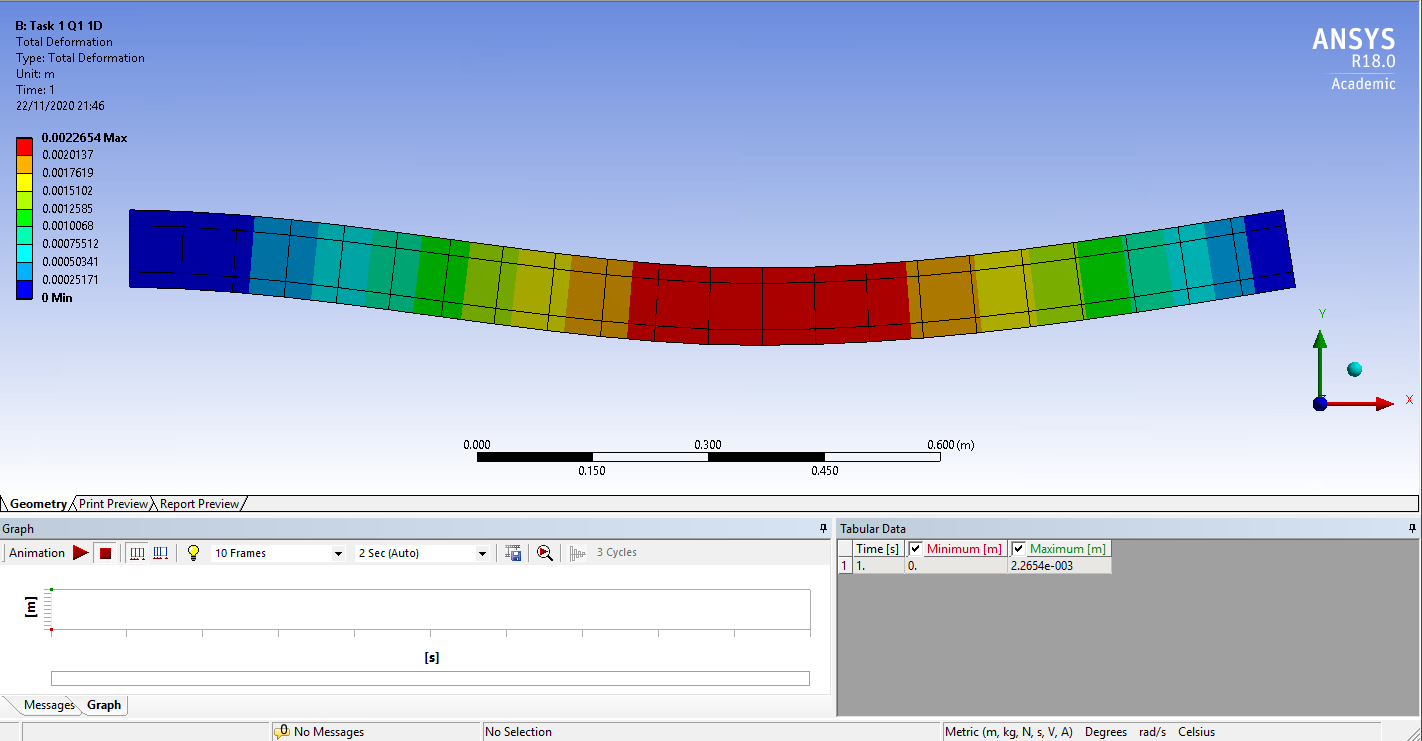
\includegraphics[width = 0.6\textwidth]{./img/TotalDeformationQ1.png}
  \caption{Total Deformation in beam}
\end{figure}
\begin{figure}[H]
  \centering
  \begin{minipage}[b]{0.49\textwidth}
    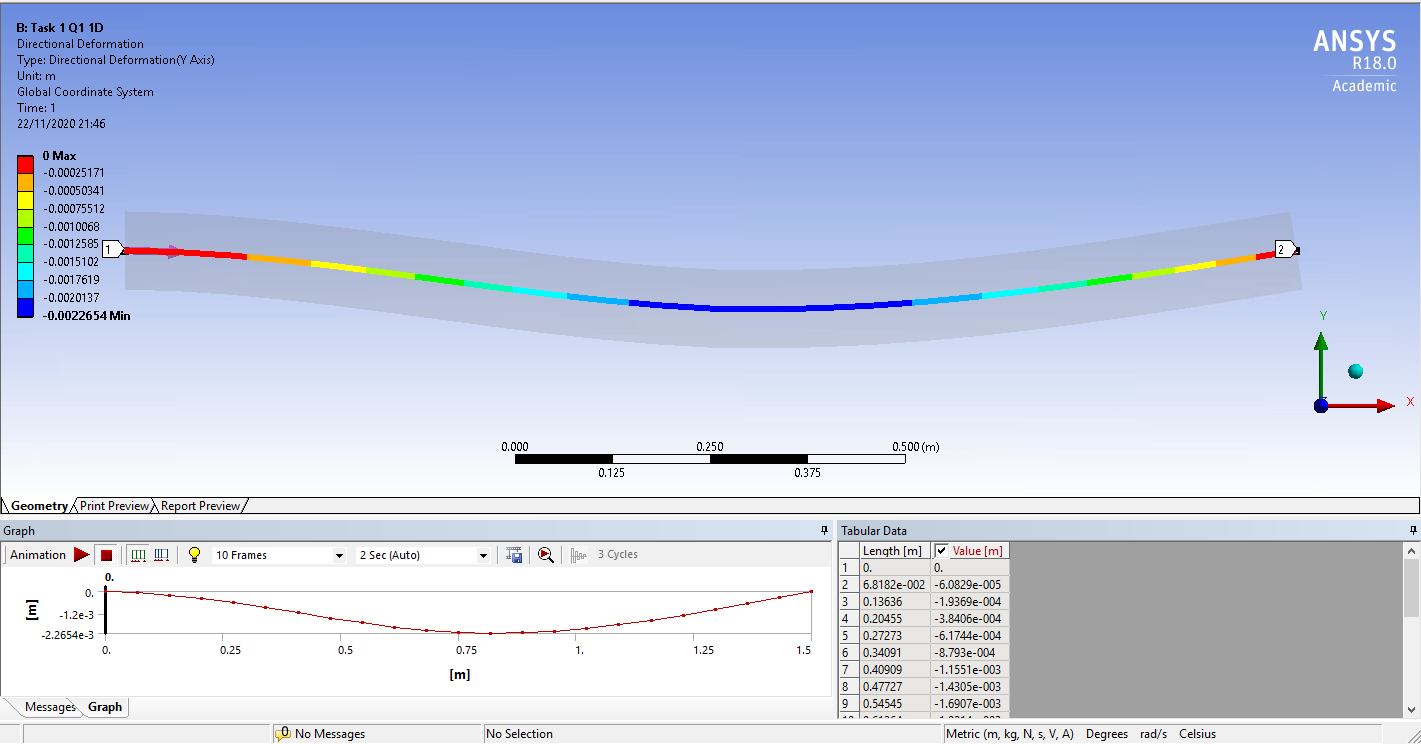
\includegraphics[width=\textwidth]{./img/DirectionalDeformationQ1.png}
    \caption{Directional Deformation in beam}
  \end{minipage}
  \hfill
  \begin{minipage}[b]{0.49\textwidth}
    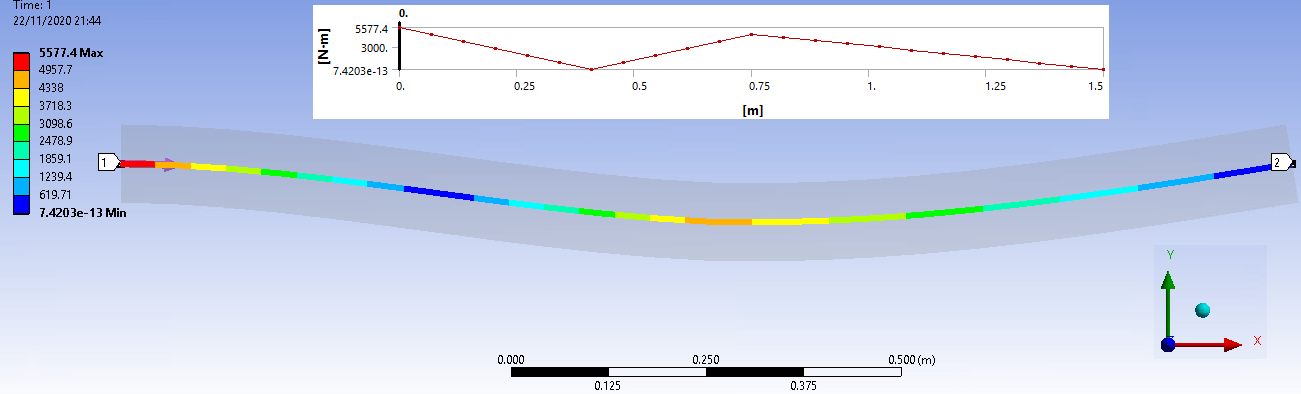
\includegraphics[width=\textwidth]{./img/BendingMomentQ1.png}
    \caption{Bending Moment in beam}
  \end{minipage}
\end{figure}
\href{https://github.com/hashadar/ME-Latex/tree/master/MECH0013/Topic%20Notes}{FIX LINK} to see numerical data of the directional deformation and the bending moment of the beam. Here, we can see that 
\end{document}